\chapter{Image Processing}
\label{cha:IP}

\section{Locating Objects}

The flowchart of whole image processing algorithm is shown in figure \ref{IP_flow}.

\begin{figure}[thb]
    \centering
    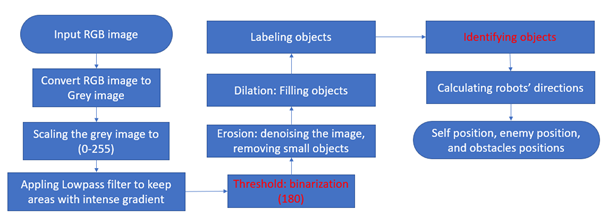
\includegraphics[width=0.8\textwidth]{images/Image processing flowchart.png}
    \caption[Image processing flowchart]{Image processing flowchart.}\label{IP_flow}
\end{figure}

While testing the code, we found if color of obstacle is changed to blue, the threshold of binarization, with original value of 80, would be not suitable anymore. After testing, the threshold is determined as 180, which is suitable for all colors of obstacles. The comparison of different thresholds is shown in figure \ref{different_threshold}.

\begin{figure}[thb]
    \centering
    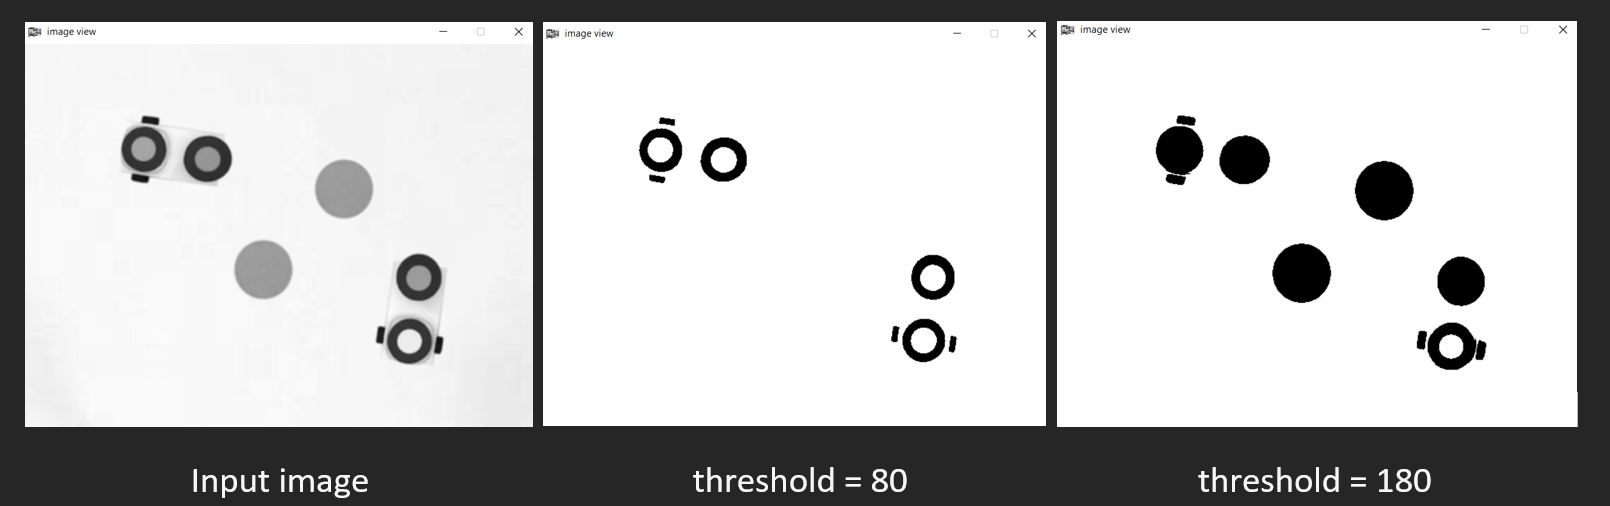
\includegraphics[width=0.8\textwidth]{images/different_threshold.png}
    \caption[Different thresholds in binarization]{Different thresholds in binarization.}\label{different_threshold}
\end{figure}

\section{Identifying Objects}

Identifying objects is the key of it, the flowchart is shown in figure \ref{Id_flow} (assume that self-robot is robot A, red and green)

\begin{figure}[thb]
    \centering
    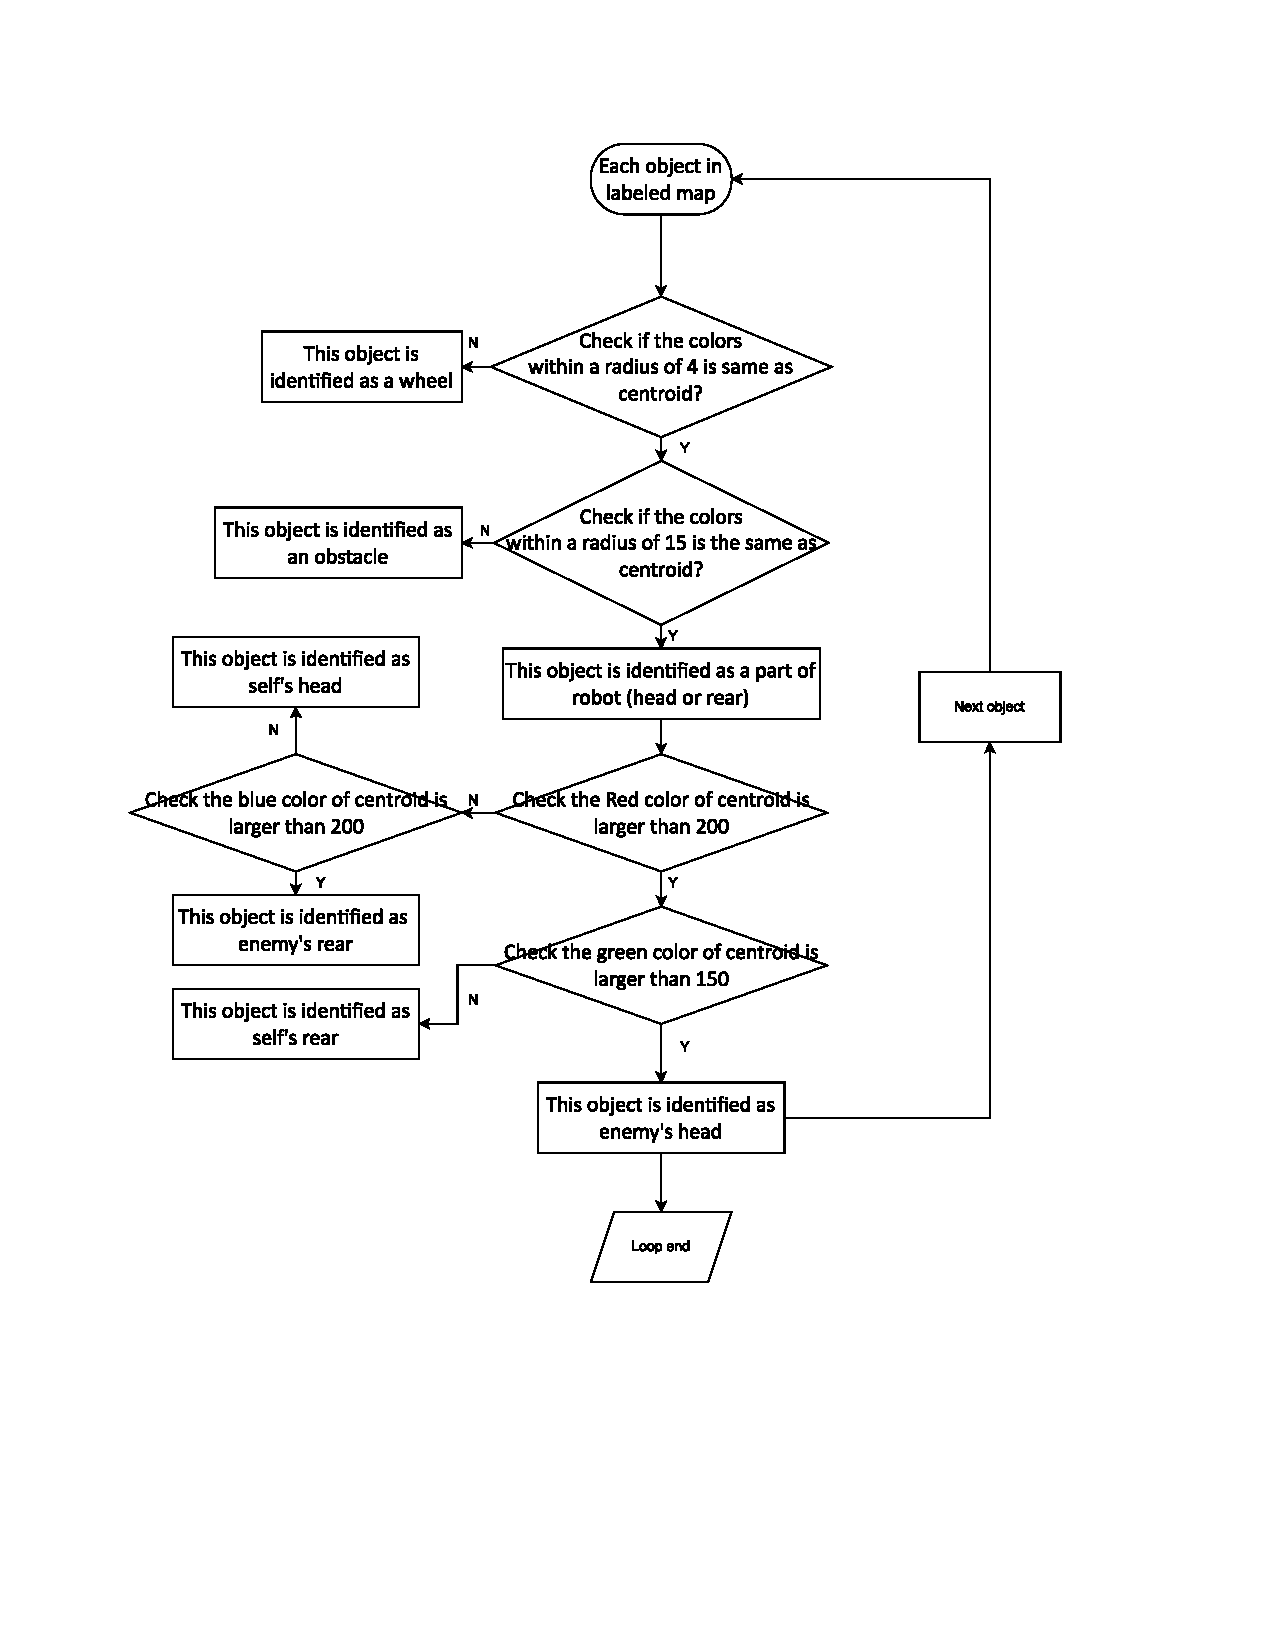
\includegraphics[width=0.75\textwidth]{images/Id_flow.pdf}
    \caption[Identifying flowchart]{Identifying flowchart.}\label{Id_flow}
\end{figure}


% \begin{table}[htbp]\small
%     \addtolength{\leftskip} {2cm}
%     \begin{tabular}{c|ccc}
%     \hline 
%     Colour&Red Value&Green Value&Blue Value\\
%     \hline 
%     Green(A1)&67&180&131\\
%     Red(A2)&226&90&77\\
%     Orange(B1)&255&189&124\\
%     Blue(B2)&48&158&228\\
%     \hline 
%     \end{tabular}
%     \caption[RGB values of four colors]{RGB values of four colors.}\label{rgb_values}
%     \end{table}

The final result of image processing is shown in figure \ref{IP_result} 
    \begin{figure}[thb]
        \centering
        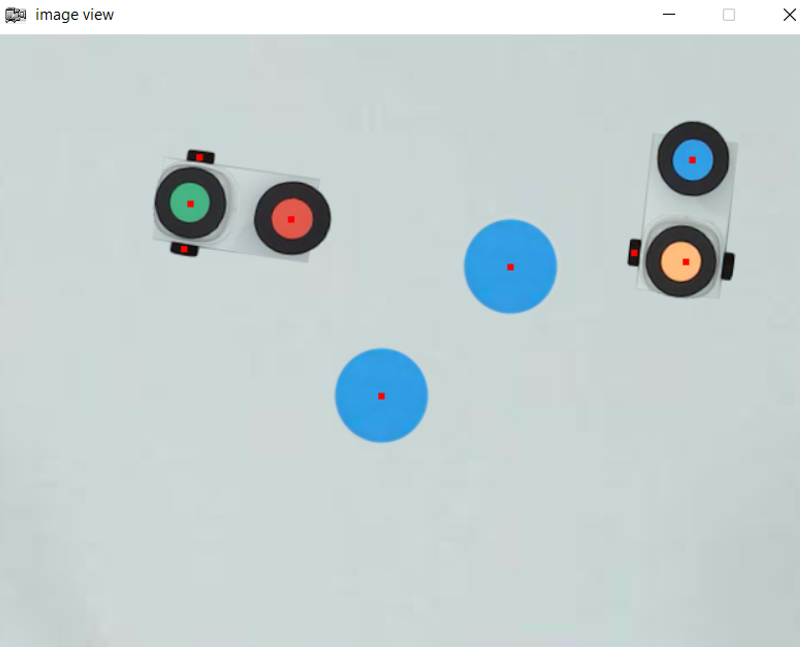
\includegraphics[width=0.6\textwidth]{images/IP_result.png}
        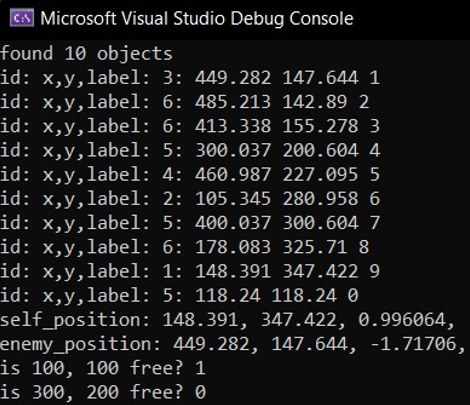
\includegraphics[width=0.6\textwidth]{images/IP_result2.png}
        \caption[Locating all objects]{Locating all objects.}\label{IP_result}
    \end{figure}
